\section{Thursday}\index{Thursday_lecture}
\paragraph{Reviewing for Probability Space}
\begin{itemize}
\item
$(\Omega,\mathcal{F},\mathbb{P})$;
\item
Random variable;
\item
Generated $\sigma$-algebra;
\end{itemize}



%A probability space is a triplet $(\Omega,\mathcal{F},\mathbb{P})$ defined as follows:
%\begin{enumerate}
%\item
%$\Omega$: denotes the probability sample space. A point $w\in\Omega$ is called a sample point
%\item
%$\mathcal{F}$: A $\sigma$-algebra $\mathcal{F}$ on $\Omega$ contains a family of events. Each event $F\in\mathcal{F}$ is an $\mathcal{F}$-measurable subset of $\Omega$.
%\begin{example}
%Let the probability space $\Omega=\{0,1,2,3\}$, then one $\mathcal{F}$ can be $\{F_1,F_2,F_3\}$, where
%\[
%\begin{array}{lll}
%F_1=\{0,1\},
%&
%F_2=\emptyset,
%&
%F_3=\{2,3\}
%\end{array}
%\]
%\end{example}
%\begin{definition}[$\sigma$-algebra]
%A $\sigma$-algebra $\mathcal{F}$ on $\Omega$ is a family of subsets of $\Omega$ such that:
%\begin{enumerate}
%\item
%$\emptyset\in\mathcal{F}$
%\item
%If $F\in\mathcal{F}$, then $F^c\in\mathcal{F}$
%\item
%If $A_n\in\mathcal{F}$ for $n\ge1$, then $\bigcup_{n=1}^\infty A_n\in\mathcal{F}$.
%\end{enumerate}
%\end{definition}
%\item
%$\mathbb{P}$ denotes a probability measure, which is a function $\mathcal{F}\to[0,1]$ such that:
%\begin{enumerate}
%\item
%$\mathbb{P}(\emptyset)=0,\mathbb{P}(\Omega)=1$.
%\item
%$\mathbb{P}$ is countably addictive, i.e., if $A_n\in\mathcal{F}$ is a countable sequence of disjoint sets, then
%\[
%\mathbb{P}\left(\bigcup_{n=1}^\infty A_n\right)=\sum_{n=1}^\infty\mathbb{P}(A_n)
%\]
%\end{enumerate}
%\begin{definition}[Almost Surely True]
%A statement $S$ is said to be \emph{almost surely true} (a.s. with probability 1), if
%\begin{enumerate}
%\item
%$F:=\{w\mid S(w)\mbox{is true}\}\in\mathcal{F}$
%\item
%$\mathbb{P}(F)=1$.
%\end{enumerate}
%\end{definition}
%\begin{definition}[Borel $\sigma$-Algebra]
%Let $\mathcal{U}$ be a collection of all open sets in a topological space $\Omega$ (e.g., $\Omega=\mathbb{R}^n$), then $\mathcal{B}(\Omega)$ denotes the \emph{smallest} $\sigma$-algebra that contains $\mathcal{U}$, which is called \emph{Borel $\sigma$-Algebra} on $\Omega$. The element $B\in\mathcal{B}(\Omega)$ is \emph{Borel subset}.
%\end{definition}
%\begin{remark}
%We usually use the notation $\mathcal{B}$ to denote $\mathcal{B}(\mathbb{R}^n)$. Here $\mathcal{B}$ contains all the open sets, all the closed sets, and all the countable unions of such sets, as well as the countable intersection of such sets.
%\end{remark}
%\begin{definition}[$\mathcal{F}$-Measurable / Random Variable]
%\begin{enumerate}
%\item
%A function $f:\Omega\to\mathbb{R}^n$ is called \emph{$\mathcal{F}$-measurable} if
%\[
%f^{-1}(\bm B)=\{w\mid f(w)\in\mathcal{B}\}\in\mathcal{F}
%\]
%for any $\bm B\in\mathcal{B}$.
%\item
%A random variable $X$ is a function $X:\Omega\to\mathbb{R}^n$ and is $\mathcal{F}$-measurable.
%\end{enumerate}
%\end{definition}
%\begin{definition}[Generated $\sigma$-Algebra]
%Suppose $X$ is a random variable on $(\Omega,\mathcal{F},\mathbb{P})$. Then the $\sigma$-algebra generated by $X$, say $\mathcal{H}_X$ is defined to be the \emph{smallest $\sigma$-algebra} on $\Omega$ containing $X^{-1}(U)$, where $U\subseteq\mathbb{R}^n$ is any open set.
%\end{definition}
\subsection{More on Probability Theory}
\begin{definition}[Distribution]
A probability measure $\mu_X$ on $\mathbb{R}^n$ induced by the random variabe $X$ isdefined as
\[
\mu_X(\bm B)=\mathbb{P}(X^{-1}(\bm B)),
\]
where $\bm B\in\mathcal{B}(\mathbb{R}^n)$. The $\mu_X$ is called the \emph{distribution} of $X$.
\end{definition}

\begin{definition}[Expectation]
The expectation of $X$ is given by
\[
\mathbb{E}[X] = \int_{\Omega}X(\omega)\diff \mathbb{P}(\omega)
\]
When $\Omega=\mathbb{R}^n$, the expectation can be written in terms of distribution function:
\[
\mathbb{E}[X] = \int_{\mathbb{R}^n}y\diff\mu_X(y)
\]
\end{definition}
Note that the expectation of the random variable $X$ is well-defined when $X$ is integrable:

\begin{definition}[Integrable]
The random variable $X$ is \emph{integrable}, if
\[
\int_\Omega|X(w)|\diff\mathbb{P}(w)<\infty.
\]
In other words, $X$ is said to be $\mathcal{L}^1$-integrable, denoted as $X\in\mathcal{L}^1(\Omega,\mathcal{F},\mathbb{P})$.
\end{definition}

\begin{example}
If $f:\mathbb{R}^n\to\mathbb{R}$ is Borel measurable, 
and $\int_{\Omega}|f(X(\omega))|\diff\mathbb{P}(\omega)<\infty$, then
\[
\mathbb{E}[f(x)] = \int_{\Omega}f(X(\omega))\diff\mathbb{P}(\omega)
=
\int_{\mathbb{R}^n}f(y)\diff\mu_X(y).
\]
\end{example}

\begin{definition}[$L^p$ space]
Suppose $X:~\Omega\to\mathbb{R}$ is a random variable and $p\ge1$.
\begin{itemize}
\item
Define $L^p$-norm of $X$ as
\[
\|X\|_p=\left(\int_\Omega|X(\omega)|^p\diff\mathbb{P}\right)^{1/p}
\]
If $p=\infty$, define
\[
\|X\|_\infty=\inf\{N\in\mathbb{R}\mid|X(w)|\le N,\text{ a.s.}\}
\]
\item
A random variable $X$ is said to be in the $L^p$ space ($p$-th integrable) if
\[
\int_\Omega|X(\omega)|^p\diff\mathbb{P}(\omega)<\infty,
\]
denoted as $X\in\mathcal{L}^p(\Omega,\mathcal{F},\mathbb{P})$.
\end{itemize}
\end{definition}


\begin{proposition}
If $p\ge q$, then $\|X\|_p\ge\|X\|_q$. Thus $\mathcal{L}^p(\Omega,\mathcal{F},\mathbb{P})\subseteq\mathcal{L}^q(\Omega,\mathcal{F},\mathbb{P})$.
\end{proposition}
\begin{proof}
The inequality is shown by using Holder's inequality:
\[
\|X\|_q^q=\int_\Omega|X|^q\diff\mathbb{P}
\le
\left(\int_\Omega(|X|^q)^{p/q}\diff\mathbb{P}\right)^{q/p}
=
\left(
\int_\Omega|X|^p\diff\mathbb{P}
\right)^{\frac{1}{p}\cdot q}
=
\|X\|_p^q.
\]
\end{proof}

Then we discuss how to define independence between two random variables, by the following three steps:
\begin{definition}[Independence]
\begin{enumerate}
\item
Two events $A_1,A_2\in\mathcal{F}$ are said to be \emph{independent} if
$
\mathbb{P}(A_1\bigcap A_2)=\mathbb{P}(A_1)\mathbb{P}(A_2).
$
\item
Two $\sigma$-algebras $\mathcal{F}_1,\mathcal{F}_2$ are said to be \emph{independent} 
if $F_1,F_2$ are independent events for $\forall F_1\in\mathcal{F}_1,F_2\in\mathcal{F}_2$
\item
Two random variables $X,Y$ are said to be \emph{independent} if $\mathcal{H}_X,\mathcal{H}_Y$, the $\sigma$-algebra generated by $X$ and $Y$, respectively, are independent.
\end{enumerate}
\end{definition}

\begin{remark}
The independence defined above can be generalized from two events 
into finite number of events.
\end{remark}

\begin{proposition}
If $X$ and $Y$ are two independent random variables,
and $\mathbb{E}[|X|]<\infty, \mathbb{E}[|Y|]<\infty$, then
\[
\mathbb{E}[XY] = \mathbb{E}[X]
\mathbb{E}[Y]<\infty.
\]
\end{proposition}
\begin{proof}
The first step is to simplify the probability distribution for the product random variable $(X,Y)$, i.e., $\mu_{X,Y}$.
\begin{remark}
From now on, we also write the event 
$\{X^{-1}(\bm B)\}$ as $\{X\in\bm B\}$ for $\bm B\in\mathcal{B}(\mathbb{R}^n)$.
\end{remark}
By the definition of independence, we have the following:
\begin{align*}
\mu_{X,Y}(A_1\times A_2)&\triangleq 
\mathbb{P}(\{(X,Y)\in (A_1\times A_2)\})
=\mathbb{P}(\{X\in A_1, Y\in A_2\})\\
&=\mathbb{P}(\{X\in A_1\})\mathbb{P}(\{Y\in A_2\})
=\mu_X(A_1)\mu_Y(A_2).
\end{align*}
Now we begin to simplify the expectation of product:
\begin{align*}
\mathbb{E}[XY]&=\int xy\diff\mu_{X,Y}(x,y)
=\iint xy\diff\mu_{X}(x)\mu_Y(y)\\
&=
\int y\bigg[
\int x\diff\mu_{X}(x)
\bigg]\mu_Y(y)=\int \mathbb{E}[X]y\mu_Y(y)=\mathbb{E}[X]\mathbb{E}[Y].
\end{align*}


\end{proof}








\subsection{Stochastic Process}

Consider a set $T$ of time index, e.g., a non-negative integer set or a time interval $[0,\infty)$.
We will discuss a discrete/continuous time stochastic process.
\begin{definition}[Stochastic Process]
A collection of random variables $\{X_t\}_{t\in T}$, defined on $(\Omega,\mathcal{F},\mathbb{P})$ and taking values in $\mathbb{R}^n$, is called a \emph{stochastic process}.
\end{definition}
\begin{remark}
A stochastic process $\{X_t\}_{t\in T}$ can also be viewed as a random function, since it is a mapping $\Omega\times T\to \mathbb{R}^n$.
Sometimes we omit the subscript to denote a stochastic process $\{X_t\}$.
\end{remark}

\begin{definition}[Sample Path]
Fixing $\omega\in\Omega$, then $\{X_t(\omega)\}_{t\in T}$~(denoted as $X_{\cdot}(\omega)$) is called a \emph{sample path}, or \emph{trajectory}. 
\end{definition}
\begin{definition}[Continuous]
A stochastic process $\{X_t\}$ is said to be \emph{continuous} (right-cot, left-cot, resp.) a.s., if
$t\to X_t(\omega)$ is \emph{continuous} (right-cot, left-cot, resp.) a.s., i.e.,
\[
\mathbb{P}
\bigg(
\{
\omega: t\to X_t(\omega)\text{ is continuous (right-cot, left-cot, resp.)}
\}
\bigg)=1.
\]
\end{definition}

\begin{example}[Poisson Process]
Consider $(\xi_j, j=1,2,\ldots)$ a sequence of i.i.d. random variables with Possion distribution with intensity $\lambda>0$.
Let $T_0=0$, and $T_n = \sum_{j=1}^n\xi_j$.
Define $X_t = n$ if $T_n \le t< T_{n+1}$.
Verify that $\{X_t\}$ is a stochastic process with right-continuity and left-limit exists.
Instead of giving a mathematical proof, we provide a numerical simulation of $\{X_t\}$ plotted in Figure.~\ref{fig:1:1}.
\footnote{The corresponding matlab code can be found in 
\[
\mbox{https://github.com/WalterBabyRudin/CourseWare/tree/master/MAT4500/week1}
\]}
\end{example}
\begin{figure}
\centering
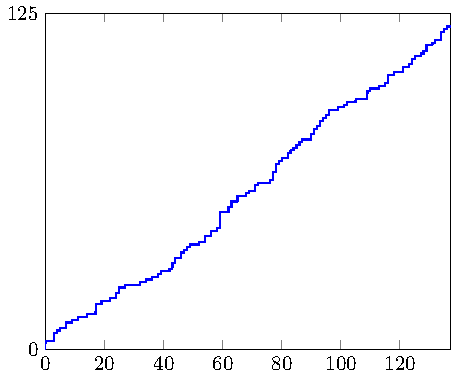
\includegraphics[width=0.7\textwidth]{week1/figure_2.pdf}
\caption{One simulation of $\{X_t\}$ with intensity $\lambda=1.2$ and $500$ samples}
\label{fig:1:1}
\end{figure}














